\section{Fixed Objects}
The user can add fixed objects by pressing the middle mouse button.
Fixed objects are maintained using a grid, that has the same size as the velocity and density grids.
If a cell contains a fixed objects the value is 1, else the value is 0.

\noindent As fixed objects consists of 5 cells, that has the structure as shown in Figure~\ref{fig:fixedstructure}.

\begin{figure}[h]
    \centering
    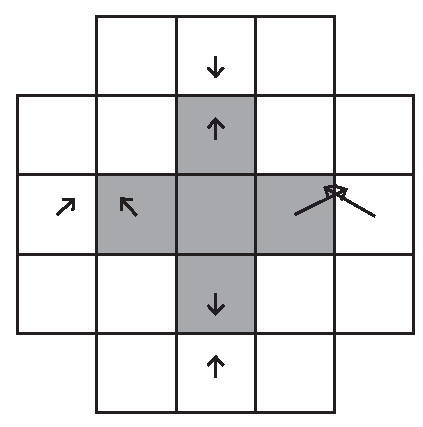
\includegraphics[width=5cm]{img/fixedstructure.pdf}
    \caption{Structure of fixed object, with boundary conditions for velocity.}
    \label{fig:fixedstructure}
\end{figure}

\noindent This structure is convenient because the velocity for each side can be calculated separately.
For example, the velocity on the top of the fixed object only uses velocity of its top neighbour.
So when a fluid is directed to the top of the fixed object, it will 'bounce' in the y-axis and remain its horizontal trajectory.
The mechanism is the same as the boundary conditions, and is also calculated the same time as the boundary conditions.

\noindent Figure~\ref{fig:fixed} shows the boundary conditions of the fixed objects. The fluid is trapped inside the square of fixed objects because it bounces back on the boundaries of the fixed objects.

\begin{figure}
    \centering
    \includegraphics[width=8cm]{img/fixed.png}
    \caption{Fluid trapped inside a square of fixed objects.}
    \label{fig:fixed}
\end{figure}
